% Created by tikzDevice version 0.12 on 2019-04-09 14:30:01
% !TEX encoding = UTF-8 Unicode
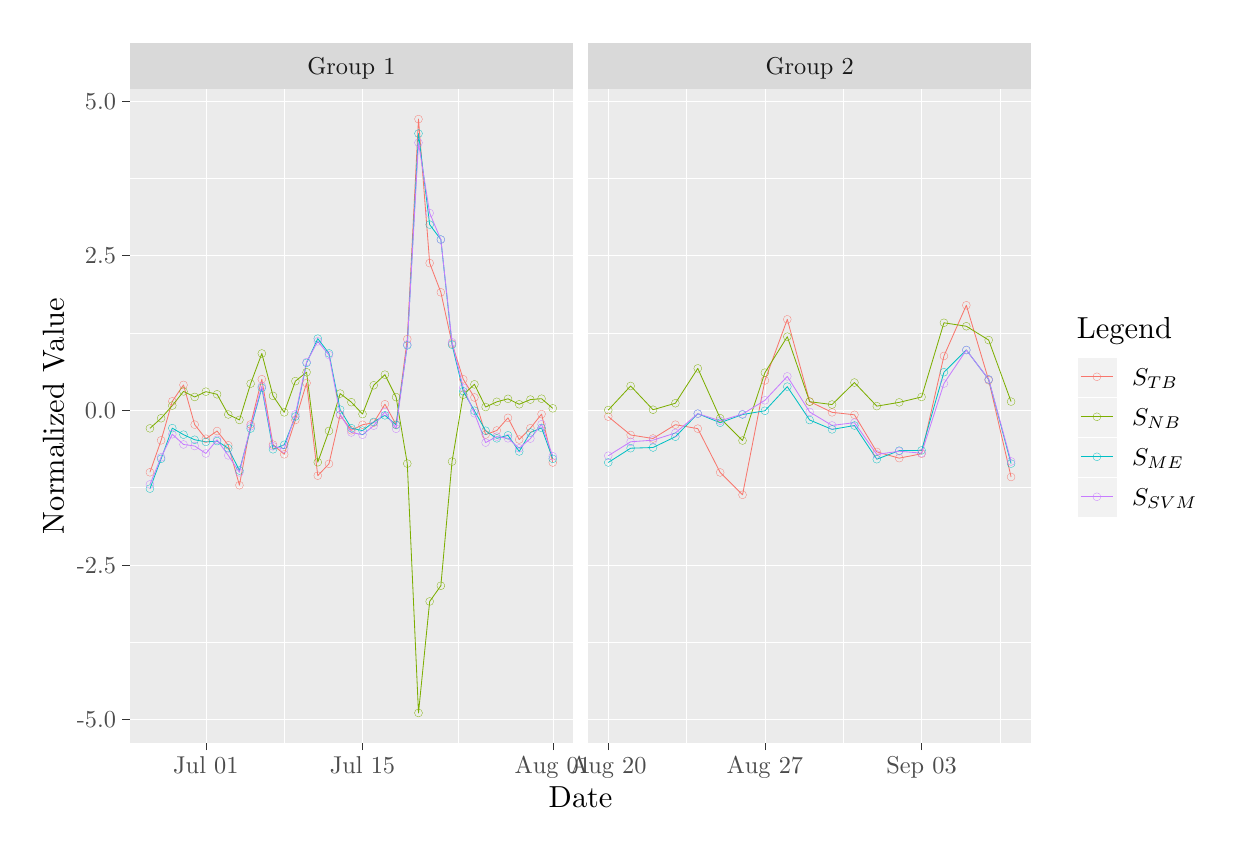
\begin{tikzpicture}[x=1pt,y=1pt]
\definecolor{fillColor}{RGB}{255,255,255}
\path[use as bounding box,fill=fillColor,fill opacity=0.00] (0,0) rectangle (433.62,289.08);
\begin{scope}
\path[clip] (  0.00,  0.00) rectangle (433.62,289.08);
\definecolor{drawColor}{RGB}{255,255,255}
\definecolor{fillColor}{RGB}{255,255,255}

\path[draw=drawColor,line width= 0.1pt,line join=round,line cap=round,fill=fillColor] (  0.00,  0.00) rectangle (433.62,289.08);
\end{scope}
\begin{scope}
\path[clip] ( 36.90, 30.73) rectangle (197.01,266.77);
\definecolor{fillColor}{gray}{0.92}

\path[fill=fillColor] ( 36.90, 30.73) rectangle (197.01,266.77);
\definecolor{drawColor}{RGB}{255,255,255}

\path[draw=drawColor,line width= 0.1pt,line join=round] ( 36.90, 67.00) --
	(197.01, 67.00);

\path[draw=drawColor,line width= 0.1pt,line join=round] ( 36.90,122.89) --
	(197.01,122.89);

\path[draw=drawColor,line width= 0.1pt,line join=round] ( 36.90,178.79) --
	(197.01,178.79);

\path[draw=drawColor,line width= 0.1pt,line join=round] ( 36.90,234.68) --
	(197.01,234.68);

\path[draw=drawColor,line width= 0.1pt,line join=round] ( 92.70, 30.73) --
	( 92.70,266.77);

\path[draw=drawColor,line width= 0.1pt,line join=round] (155.37, 30.73) --
	(155.37,266.77);

\path[draw=drawColor,line width= 0.1pt,line join=round] ( 36.90, 39.05) --
	(197.01, 39.05);

\path[draw=drawColor,line width= 0.1pt,line join=round] ( 36.90, 94.95) --
	(197.01, 94.95);

\path[draw=drawColor,line width= 0.1pt,line join=round] ( 36.90,150.84) --
	(197.01,150.84);

\path[draw=drawColor,line width= 0.1pt,line join=round] ( 36.90,206.73) --
	(197.01,206.73);

\path[draw=drawColor,line width= 0.1pt,line join=round] ( 36.90,262.63) --
	(197.01,262.63);

\path[draw=drawColor,line width= 0.1pt,line join=round] ( 64.39, 30.73) --
	( 64.39,266.77);

\path[draw=drawColor,line width= 0.1pt,line join=round] (121.00, 30.73) --
	(121.00,266.77);

\path[draw=drawColor,line width= 0.1pt,line join=round] (189.74, 30.73) --
	(189.74,266.77);
\definecolor{drawColor}{RGB}{248,118,109}

\path[draw=drawColor,line width= 0.3pt,line join=round] ( 44.18,128.42) --
	( 48.22,139.97) --
	( 52.26,154.07) --
	( 56.31,159.99) --
	( 60.35,145.63) --
	( 64.39,140.54) --
	( 68.44,143.33) --
	( 72.48,138.19) --
	( 76.52,123.74) --
	( 80.57,145.71) --
	( 84.61,162.05) --
	( 88.65,138.42) --
	( 92.70,134.91) --
	( 96.74,147.31) --
	(100.78,160.65) --
	(104.83,127.19) --
	(108.87,131.47) --
	(112.91,149.12) --
	(116.96,143.59) --
	(121.00,145.58) --
	(125.04,146.35) --
	(129.09,153.00) --
	(133.13,145.64) --
	(137.17,176.53) --
	(141.22,256.04) --
	(145.26,204.01) --
	(149.30,193.46) --
	(153.35,174.91) --
	(157.39,162.04) --
	(161.43,155.46) --
	(165.48,142.05) --
	(169.52,143.52) --
	(173.56,148.10) --
	(177.61,140.24) --
	(181.65,144.34) --
	(185.69,149.44) --
	(189.74,131.95);
\definecolor{drawColor}{RGB}{124,174,0}

\path[draw=drawColor,line width= 0.3pt,line join=round] ( 44.18,144.29) --
	( 48.22,147.95) --
	( 52.26,152.52) --
	( 56.31,157.64) --
	( 60.35,155.64) --
	( 64.39,157.55) --
	( 68.44,156.60) --
	( 72.48,149.32) --
	( 76.52,147.34) --
	( 80.57,160.45) --
	( 84.61,171.34) --
	( 88.65,156.03) --
	( 92.70,150.08) --
	( 96.74,161.36) --
	(100.78,164.58) --
	(104.83,132.05) --
	(108.87,143.36) --
	(112.91,156.86) --
	(116.96,153.75) --
	(121.00,149.45) --
	(125.04,159.86) --
	(129.09,163.69) --
	(133.13,155.58) --
	(137.17,131.56) --
	(141.22, 41.46) --
	(145.26, 81.74) --
	(149.30, 87.42) --
	(153.35,132.29) --
	(157.39,156.46) --
	(161.43,160.20) --
	(165.48,151.99) --
	(169.52,153.88) --
	(173.56,154.96) --
	(177.61,152.99) --
	(181.65,154.69) --
	(185.69,155.01) --
	(189.74,151.53);
\definecolor{drawColor}{RGB}{0,191,196}

\path[draw=drawColor,line width= 0.3pt,line join=round] ( 44.18,122.50) --
	( 48.22,133.29) --
	( 52.26,144.37) --
	( 56.31,142.01) --
	( 60.35,140.17) --
	( 64.39,139.40) --
	( 68.44,139.69) --
	( 72.48,137.11) --
	( 76.52,129.05) --
	( 80.57,144.24) --
	( 84.61,158.93) --
	( 88.65,136.73) --
	( 92.70,138.35) --
	( 96.74,148.58) --
	(100.78,167.95) --
	(104.83,176.71) --
	(108.87,171.39) --
	(112.91,151.05) --
	(116.96,144.35) --
	(121.00,143.47) --
	(125.04,146.61) --
	(129.09,149.00) --
	(133.13,145.50) --
	(137.17,174.28) --
	(141.22,250.81) --
	(145.26,217.91) --
	(149.30,212.52) --
	(153.35,174.52) --
	(157.39,157.70) --
	(161.43,150.66) --
	(165.48,143.43) --
	(169.52,140.68) --
	(173.56,141.78) --
	(177.61,135.94) --
	(181.65,142.79) --
	(185.69,144.46) --
	(189.74,133.28);
\definecolor{drawColor}{RGB}{199,124,255}

\path[draw=drawColor,line width= 0.3pt,line join=round] ( 44.18,124.04) --
	( 48.22,133.83) --
	( 52.26,142.17) --
	( 56.31,138.47) --
	( 60.35,137.91) --
	( 64.39,135.21) --
	( 68.44,140.14) --
	( 72.48,134.53) --
	( 76.52,128.40) --
	( 80.57,145.03) --
	( 84.61,159.51) --
	( 88.65,137.80) --
	( 92.70,136.92) --
	( 96.74,149.36) --
	(100.78,168.23) --
	(104.83,175.74) --
	(108.87,170.80) --
	(112.91,149.30) --
	(116.96,142.81) --
	(121.00,141.98) --
	(125.04,145.26) --
	(129.09,150.23) --
	(133.13,144.14) --
	(137.17,174.61) --
	(141.22,247.51) --
	(145.26,222.08) --
	(149.30,212.47) --
	(153.35,175.40) --
	(157.39,158.96) --
	(161.43,149.76) --
	(165.48,139.15) --
	(169.52,141.31) --
	(173.56,140.70) --
	(177.61,137.09) --
	(181.65,140.60) --
	(185.69,145.78) --
	(189.74,134.21);
\definecolor{drawColor}{RGB}{248,118,109}

\path[draw=drawColor,line width= 0.1pt,line join=round,line cap=round] ( 44.18,128.42) circle (  1.43);

\path[draw=drawColor,line width= 0.1pt,line join=round,line cap=round] ( 48.22,139.97) circle (  1.43);

\path[draw=drawColor,line width= 0.1pt,line join=round,line cap=round] ( 52.26,154.07) circle (  1.43);

\path[draw=drawColor,line width= 0.1pt,line join=round,line cap=round] ( 56.31,159.99) circle (  1.43);

\path[draw=drawColor,line width= 0.1pt,line join=round,line cap=round] ( 60.35,145.63) circle (  1.43);

\path[draw=drawColor,line width= 0.1pt,line join=round,line cap=round] ( 64.39,140.54) circle (  1.43);

\path[draw=drawColor,line width= 0.1pt,line join=round,line cap=round] ( 68.44,143.33) circle (  1.43);

\path[draw=drawColor,line width= 0.1pt,line join=round,line cap=round] ( 72.48,138.19) circle (  1.43);

\path[draw=drawColor,line width= 0.1pt,line join=round,line cap=round] ( 76.52,123.74) circle (  1.43);

\path[draw=drawColor,line width= 0.1pt,line join=round,line cap=round] ( 80.57,145.71) circle (  1.43);

\path[draw=drawColor,line width= 0.1pt,line join=round,line cap=round] ( 84.61,162.05) circle (  1.43);

\path[draw=drawColor,line width= 0.1pt,line join=round,line cap=round] ( 88.65,138.42) circle (  1.43);

\path[draw=drawColor,line width= 0.1pt,line join=round,line cap=round] ( 92.70,134.91) circle (  1.43);

\path[draw=drawColor,line width= 0.1pt,line join=round,line cap=round] ( 96.74,147.31) circle (  1.43);

\path[draw=drawColor,line width= 0.1pt,line join=round,line cap=round] (100.78,160.65) circle (  1.43);

\path[draw=drawColor,line width= 0.1pt,line join=round,line cap=round] (104.83,127.19) circle (  1.43);

\path[draw=drawColor,line width= 0.1pt,line join=round,line cap=round] (108.87,131.47) circle (  1.43);

\path[draw=drawColor,line width= 0.1pt,line join=round,line cap=round] (112.91,149.12) circle (  1.43);

\path[draw=drawColor,line width= 0.1pt,line join=round,line cap=round] (116.96,143.59) circle (  1.43);

\path[draw=drawColor,line width= 0.1pt,line join=round,line cap=round] (121.00,145.58) circle (  1.43);

\path[draw=drawColor,line width= 0.1pt,line join=round,line cap=round] (125.04,146.35) circle (  1.43);

\path[draw=drawColor,line width= 0.1pt,line join=round,line cap=round] (129.09,153.00) circle (  1.43);

\path[draw=drawColor,line width= 0.1pt,line join=round,line cap=round] (133.13,145.64) circle (  1.43);

\path[draw=drawColor,line width= 0.1pt,line join=round,line cap=round] (137.17,176.53) circle (  1.43);

\path[draw=drawColor,line width= 0.1pt,line join=round,line cap=round] (141.22,256.04) circle (  1.43);

\path[draw=drawColor,line width= 0.1pt,line join=round,line cap=round] (145.26,204.01) circle (  1.43);

\path[draw=drawColor,line width= 0.1pt,line join=round,line cap=round] (149.30,193.46) circle (  1.43);

\path[draw=drawColor,line width= 0.1pt,line join=round,line cap=round] (153.35,174.91) circle (  1.43);

\path[draw=drawColor,line width= 0.1pt,line join=round,line cap=round] (157.39,162.04) circle (  1.43);

\path[draw=drawColor,line width= 0.1pt,line join=round,line cap=round] (161.43,155.46) circle (  1.43);

\path[draw=drawColor,line width= 0.1pt,line join=round,line cap=round] (165.48,142.05) circle (  1.43);

\path[draw=drawColor,line width= 0.1pt,line join=round,line cap=round] (169.52,143.52) circle (  1.43);

\path[draw=drawColor,line width= 0.1pt,line join=round,line cap=round] (173.56,148.10) circle (  1.43);

\path[draw=drawColor,line width= 0.1pt,line join=round,line cap=round] (177.61,140.24) circle (  1.43);

\path[draw=drawColor,line width= 0.1pt,line join=round,line cap=round] (181.65,144.34) circle (  1.43);

\path[draw=drawColor,line width= 0.1pt,line join=round,line cap=round] (185.69,149.44) circle (  1.43);

\path[draw=drawColor,line width= 0.1pt,line join=round,line cap=round] (189.74,131.95) circle (  1.43);
\definecolor{drawColor}{RGB}{124,174,0}

\path[draw=drawColor,line width= 0.1pt,line join=round,line cap=round] ( 44.18,144.29) circle (  1.43);

\path[draw=drawColor,line width= 0.1pt,line join=round,line cap=round] ( 48.22,147.95) circle (  1.43);

\path[draw=drawColor,line width= 0.1pt,line join=round,line cap=round] ( 52.26,152.52) circle (  1.43);

\path[draw=drawColor,line width= 0.1pt,line join=round,line cap=round] ( 56.31,157.64) circle (  1.43);

\path[draw=drawColor,line width= 0.1pt,line join=round,line cap=round] ( 60.35,155.64) circle (  1.43);

\path[draw=drawColor,line width= 0.1pt,line join=round,line cap=round] ( 64.39,157.55) circle (  1.43);

\path[draw=drawColor,line width= 0.1pt,line join=round,line cap=round] ( 68.44,156.60) circle (  1.43);

\path[draw=drawColor,line width= 0.1pt,line join=round,line cap=round] ( 72.48,149.32) circle (  1.43);

\path[draw=drawColor,line width= 0.1pt,line join=round,line cap=round] ( 76.52,147.34) circle (  1.43);

\path[draw=drawColor,line width= 0.1pt,line join=round,line cap=round] ( 80.57,160.45) circle (  1.43);

\path[draw=drawColor,line width= 0.1pt,line join=round,line cap=round] ( 84.61,171.34) circle (  1.43);

\path[draw=drawColor,line width= 0.1pt,line join=round,line cap=round] ( 88.65,156.03) circle (  1.43);

\path[draw=drawColor,line width= 0.1pt,line join=round,line cap=round] ( 92.70,150.08) circle (  1.43);

\path[draw=drawColor,line width= 0.1pt,line join=round,line cap=round] ( 96.74,161.36) circle (  1.43);

\path[draw=drawColor,line width= 0.1pt,line join=round,line cap=round] (100.78,164.58) circle (  1.43);

\path[draw=drawColor,line width= 0.1pt,line join=round,line cap=round] (104.83,132.05) circle (  1.43);

\path[draw=drawColor,line width= 0.1pt,line join=round,line cap=round] (108.87,143.36) circle (  1.43);

\path[draw=drawColor,line width= 0.1pt,line join=round,line cap=round] (112.91,156.86) circle (  1.43);

\path[draw=drawColor,line width= 0.1pt,line join=round,line cap=round] (116.96,153.75) circle (  1.43);

\path[draw=drawColor,line width= 0.1pt,line join=round,line cap=round] (121.00,149.45) circle (  1.43);

\path[draw=drawColor,line width= 0.1pt,line join=round,line cap=round] (125.04,159.86) circle (  1.43);

\path[draw=drawColor,line width= 0.1pt,line join=round,line cap=round] (129.09,163.69) circle (  1.43);

\path[draw=drawColor,line width= 0.1pt,line join=round,line cap=round] (133.13,155.58) circle (  1.43);

\path[draw=drawColor,line width= 0.1pt,line join=round,line cap=round] (137.17,131.56) circle (  1.43);

\path[draw=drawColor,line width= 0.1pt,line join=round,line cap=round] (141.22, 41.46) circle (  1.43);

\path[draw=drawColor,line width= 0.1pt,line join=round,line cap=round] (145.26, 81.74) circle (  1.43);

\path[draw=drawColor,line width= 0.1pt,line join=round,line cap=round] (149.30, 87.42) circle (  1.43);

\path[draw=drawColor,line width= 0.1pt,line join=round,line cap=round] (153.35,132.29) circle (  1.43);

\path[draw=drawColor,line width= 0.1pt,line join=round,line cap=round] (157.39,156.46) circle (  1.43);

\path[draw=drawColor,line width= 0.1pt,line join=round,line cap=round] (161.43,160.20) circle (  1.43);

\path[draw=drawColor,line width= 0.1pt,line join=round,line cap=round] (165.48,151.99) circle (  1.43);

\path[draw=drawColor,line width= 0.1pt,line join=round,line cap=round] (169.52,153.88) circle (  1.43);

\path[draw=drawColor,line width= 0.1pt,line join=round,line cap=round] (173.56,154.96) circle (  1.43);

\path[draw=drawColor,line width= 0.1pt,line join=round,line cap=round] (177.61,152.99) circle (  1.43);

\path[draw=drawColor,line width= 0.1pt,line join=round,line cap=round] (181.65,154.69) circle (  1.43);

\path[draw=drawColor,line width= 0.1pt,line join=round,line cap=round] (185.69,155.01) circle (  1.43);

\path[draw=drawColor,line width= 0.1pt,line join=round,line cap=round] (189.74,151.53) circle (  1.43);
\definecolor{drawColor}{RGB}{0,191,196}

\path[draw=drawColor,line width= 0.1pt,line join=round,line cap=round] ( 44.18,122.50) circle (  1.43);

\path[draw=drawColor,line width= 0.1pt,line join=round,line cap=round] ( 48.22,133.29) circle (  1.43);

\path[draw=drawColor,line width= 0.1pt,line join=round,line cap=round] ( 52.26,144.37) circle (  1.43);

\path[draw=drawColor,line width= 0.1pt,line join=round,line cap=round] ( 56.31,142.01) circle (  1.43);

\path[draw=drawColor,line width= 0.1pt,line join=round,line cap=round] ( 60.35,140.17) circle (  1.43);

\path[draw=drawColor,line width= 0.1pt,line join=round,line cap=round] ( 64.39,139.40) circle (  1.43);

\path[draw=drawColor,line width= 0.1pt,line join=round,line cap=round] ( 68.44,139.69) circle (  1.43);

\path[draw=drawColor,line width= 0.1pt,line join=round,line cap=round] ( 72.48,137.11) circle (  1.43);

\path[draw=drawColor,line width= 0.1pt,line join=round,line cap=round] ( 76.52,129.05) circle (  1.43);

\path[draw=drawColor,line width= 0.1pt,line join=round,line cap=round] ( 80.57,144.24) circle (  1.43);

\path[draw=drawColor,line width= 0.1pt,line join=round,line cap=round] ( 84.61,158.93) circle (  1.43);

\path[draw=drawColor,line width= 0.1pt,line join=round,line cap=round] ( 88.65,136.73) circle (  1.43);

\path[draw=drawColor,line width= 0.1pt,line join=round,line cap=round] ( 92.70,138.35) circle (  1.43);

\path[draw=drawColor,line width= 0.1pt,line join=round,line cap=round] ( 96.74,148.58) circle (  1.43);

\path[draw=drawColor,line width= 0.1pt,line join=round,line cap=round] (100.78,167.95) circle (  1.43);

\path[draw=drawColor,line width= 0.1pt,line join=round,line cap=round] (104.83,176.71) circle (  1.43);

\path[draw=drawColor,line width= 0.1pt,line join=round,line cap=round] (108.87,171.39) circle (  1.43);

\path[draw=drawColor,line width= 0.1pt,line join=round,line cap=round] (112.91,151.05) circle (  1.43);

\path[draw=drawColor,line width= 0.1pt,line join=round,line cap=round] (116.96,144.35) circle (  1.43);

\path[draw=drawColor,line width= 0.1pt,line join=round,line cap=round] (121.00,143.47) circle (  1.43);

\path[draw=drawColor,line width= 0.1pt,line join=round,line cap=round] (125.04,146.61) circle (  1.43);

\path[draw=drawColor,line width= 0.1pt,line join=round,line cap=round] (129.09,149.00) circle (  1.43);

\path[draw=drawColor,line width= 0.1pt,line join=round,line cap=round] (133.13,145.50) circle (  1.43);

\path[draw=drawColor,line width= 0.1pt,line join=round,line cap=round] (137.17,174.28) circle (  1.43);

\path[draw=drawColor,line width= 0.1pt,line join=round,line cap=round] (141.22,250.81) circle (  1.43);

\path[draw=drawColor,line width= 0.1pt,line join=round,line cap=round] (145.26,217.91) circle (  1.43);

\path[draw=drawColor,line width= 0.1pt,line join=round,line cap=round] (149.30,212.52) circle (  1.43);

\path[draw=drawColor,line width= 0.1pt,line join=round,line cap=round] (153.35,174.52) circle (  1.43);

\path[draw=drawColor,line width= 0.1pt,line join=round,line cap=round] (157.39,157.70) circle (  1.43);

\path[draw=drawColor,line width= 0.1pt,line join=round,line cap=round] (161.43,150.66) circle (  1.43);

\path[draw=drawColor,line width= 0.1pt,line join=round,line cap=round] (165.48,143.43) circle (  1.43);

\path[draw=drawColor,line width= 0.1pt,line join=round,line cap=round] (169.52,140.68) circle (  1.43);

\path[draw=drawColor,line width= 0.1pt,line join=round,line cap=round] (173.56,141.78) circle (  1.43);

\path[draw=drawColor,line width= 0.1pt,line join=round,line cap=round] (177.61,135.94) circle (  1.43);

\path[draw=drawColor,line width= 0.1pt,line join=round,line cap=round] (181.65,142.79) circle (  1.43);

\path[draw=drawColor,line width= 0.1pt,line join=round,line cap=round] (185.69,144.46) circle (  1.43);

\path[draw=drawColor,line width= 0.1pt,line join=round,line cap=round] (189.74,133.28) circle (  1.43);
\definecolor{drawColor}{RGB}{199,124,255}

\path[draw=drawColor,line width= 0.1pt,line join=round,line cap=round] ( 44.18,124.04) circle (  1.43);

\path[draw=drawColor,line width= 0.1pt,line join=round,line cap=round] ( 48.22,133.83) circle (  1.43);

\path[draw=drawColor,line width= 0.1pt,line join=round,line cap=round] ( 52.26,142.17) circle (  1.43);

\path[draw=drawColor,line width= 0.1pt,line join=round,line cap=round] ( 56.31,138.47) circle (  1.43);

\path[draw=drawColor,line width= 0.1pt,line join=round,line cap=round] ( 60.35,137.91) circle (  1.43);

\path[draw=drawColor,line width= 0.1pt,line join=round,line cap=round] ( 64.39,135.21) circle (  1.43);

\path[draw=drawColor,line width= 0.1pt,line join=round,line cap=round] ( 68.44,140.14) circle (  1.43);

\path[draw=drawColor,line width= 0.1pt,line join=round,line cap=round] ( 72.48,134.53) circle (  1.43);

\path[draw=drawColor,line width= 0.1pt,line join=round,line cap=round] ( 76.52,128.40) circle (  1.43);

\path[draw=drawColor,line width= 0.1pt,line join=round,line cap=round] ( 80.57,145.03) circle (  1.43);

\path[draw=drawColor,line width= 0.1pt,line join=round,line cap=round] ( 84.61,159.51) circle (  1.43);

\path[draw=drawColor,line width= 0.1pt,line join=round,line cap=round] ( 88.65,137.80) circle (  1.43);

\path[draw=drawColor,line width= 0.1pt,line join=round,line cap=round] ( 92.70,136.92) circle (  1.43);

\path[draw=drawColor,line width= 0.1pt,line join=round,line cap=round] ( 96.74,149.36) circle (  1.43);

\path[draw=drawColor,line width= 0.1pt,line join=round,line cap=round] (100.78,168.23) circle (  1.43);

\path[draw=drawColor,line width= 0.1pt,line join=round,line cap=round] (104.83,175.74) circle (  1.43);

\path[draw=drawColor,line width= 0.1pt,line join=round,line cap=round] (108.87,170.80) circle (  1.43);

\path[draw=drawColor,line width= 0.1pt,line join=round,line cap=round] (112.91,149.30) circle (  1.43);

\path[draw=drawColor,line width= 0.1pt,line join=round,line cap=round] (116.96,142.81) circle (  1.43);

\path[draw=drawColor,line width= 0.1pt,line join=round,line cap=round] (121.00,141.98) circle (  1.43);

\path[draw=drawColor,line width= 0.1pt,line join=round,line cap=round] (125.04,145.26) circle (  1.43);

\path[draw=drawColor,line width= 0.1pt,line join=round,line cap=round] (129.09,150.23) circle (  1.43);

\path[draw=drawColor,line width= 0.1pt,line join=round,line cap=round] (133.13,144.14) circle (  1.43);

\path[draw=drawColor,line width= 0.1pt,line join=round,line cap=round] (137.17,174.61) circle (  1.43);

\path[draw=drawColor,line width= 0.1pt,line join=round,line cap=round] (141.22,247.51) circle (  1.43);

\path[draw=drawColor,line width= 0.1pt,line join=round,line cap=round] (145.26,222.08) circle (  1.43);

\path[draw=drawColor,line width= 0.1pt,line join=round,line cap=round] (149.30,212.47) circle (  1.43);

\path[draw=drawColor,line width= 0.1pt,line join=round,line cap=round] (153.35,175.40) circle (  1.43);

\path[draw=drawColor,line width= 0.1pt,line join=round,line cap=round] (157.39,158.96) circle (  1.43);

\path[draw=drawColor,line width= 0.1pt,line join=round,line cap=round] (161.43,149.76) circle (  1.43);

\path[draw=drawColor,line width= 0.1pt,line join=round,line cap=round] (165.48,139.15) circle (  1.43);

\path[draw=drawColor,line width= 0.1pt,line join=round,line cap=round] (169.52,141.31) circle (  1.43);

\path[draw=drawColor,line width= 0.1pt,line join=round,line cap=round] (173.56,140.70) circle (  1.43);

\path[draw=drawColor,line width= 0.1pt,line join=round,line cap=round] (177.61,137.09) circle (  1.43);

\path[draw=drawColor,line width= 0.1pt,line join=round,line cap=round] (181.65,140.60) circle (  1.43);

\path[draw=drawColor,line width= 0.1pt,line join=round,line cap=round] (185.69,145.78) circle (  1.43);

\path[draw=drawColor,line width= 0.1pt,line join=round,line cap=round] (189.74,134.21) circle (  1.43);
\end{scope}
\begin{scope}
\path[clip] (202.51, 30.73) rectangle (362.63,266.77);
\definecolor{fillColor}{gray}{0.92}

\path[fill=fillColor] (202.51, 30.73) rectangle (362.63,266.77);
\definecolor{drawColor}{RGB}{255,255,255}

\path[draw=drawColor,line width= 0.1pt,line join=round] (202.51, 67.00) --
	(362.63, 67.00);

\path[draw=drawColor,line width= 0.1pt,line join=round] (202.51,122.89) --
	(362.63,122.89);

\path[draw=drawColor,line width= 0.1pt,line join=round] (202.51,178.79) --
	(362.63,178.79);

\path[draw=drawColor,line width= 0.1pt,line join=round] (202.51,234.68) --
	(362.63,234.68);

\path[draw=drawColor,line width= 0.1pt,line join=round] (238.10, 30.73) --
	(238.10,266.77);

\path[draw=drawColor,line width= 0.1pt,line join=round] (294.70, 30.73) --
	(294.70,266.77);

\path[draw=drawColor,line width= 0.1pt,line join=round] (351.31, 30.73) --
	(351.31,266.77);

\path[draw=drawColor,line width= 0.1pt,line join=round] (202.51, 39.05) --
	(362.63, 39.05);

\path[draw=drawColor,line width= 0.1pt,line join=round] (202.51, 94.95) --
	(362.63, 94.95);

\path[draw=drawColor,line width= 0.1pt,line join=round] (202.51,150.84) --
	(362.63,150.84);

\path[draw=drawColor,line width= 0.1pt,line join=round] (202.51,206.73) --
	(362.63,206.73);

\path[draw=drawColor,line width= 0.1pt,line join=round] (202.51,262.63) --
	(362.63,262.63);

\path[draw=drawColor,line width= 0.1pt,line join=round] (209.79, 30.73) --
	(209.79,266.77);

\path[draw=drawColor,line width= 0.1pt,line join=round] (266.40, 30.73) --
	(266.40,266.77);

\path[draw=drawColor,line width= 0.1pt,line join=round] (323.01, 30.73) --
	(323.01,266.77);
\definecolor{drawColor}{RGB}{248,118,109}

\path[draw=drawColor,line width= 0.3pt,line join=round] (209.79,148.53) --
	(217.88,141.90) --
	(225.97,140.62) --
	(234.05,145.62) --
	(242.14,144.19) --
	(250.23,128.36) --
	(258.31,120.27) --
	(266.40,161.61) --
	(274.49,183.68) --
	(282.57,153.97) --
	(290.66,150.08) --
	(298.75,149.18) --
	(306.83,135.78) --
	(314.92,133.52) --
	(323.01,135.12) --
	(331.09,170.45) --
	(339.18,188.77) --
	(347.26,161.68) --
	(355.35,126.72);
\definecolor{drawColor}{RGB}{124,174,0}

\path[draw=drawColor,line width= 0.3pt,line join=round] (209.79,150.90) --
	(217.88,159.60) --
	(225.97,151.02) --
	(234.05,153.37) --
	(242.14,165.96) --
	(250.23,147.96) --
	(258.31,139.88) --
	(266.40,164.41) --
	(274.49,177.42) --
	(282.57,153.92) --
	(290.66,152.90) --
	(298.75,160.84) --
	(306.83,152.32) --
	(314.92,153.68) --
	(323.01,155.63) --
	(331.09,182.44) --
	(339.18,181.19) --
	(347.26,176.19) --
	(355.35,153.95);
\definecolor{drawColor}{RGB}{0,191,196}

\path[draw=drawColor,line width= 0.3pt,line join=round] (209.79,131.96) --
	(217.88,137.12) --
	(225.97,137.37) --
	(234.05,141.27) --
	(242.14,149.60) --
	(250.23,146.32) --
	(258.31,149.29) --
	(266.40,150.64) --
	(274.49,159.37) --
	(282.57,147.30) --
	(290.66,143.91) --
	(298.75,145.32) --
	(306.83,133.14) --
	(314.92,136.24) --
	(323.01,136.33) --
	(331.09,164.58) --
	(339.18,172.61) --
	(347.26,161.95) --
	(355.35,131.55);
\definecolor{drawColor}{RGB}{199,124,255}

\path[draw=drawColor,line width= 0.3pt,line join=round] (209.79,134.40) --
	(217.88,139.44) --
	(225.97,140.02) --
	(234.05,142.62) --
	(242.14,149.61) --
	(250.23,147.02) --
	(258.31,149.45) --
	(266.40,154.43) --
	(274.49,163.07) --
	(282.57,150.21) --
	(290.66,145.35) --
	(298.75,146.35) --
	(306.83,134.88) --
	(314.92,136.03) --
	(323.01,135.33) --
	(331.09,160.49) --
	(339.18,172.58) --
	(347.26,162.00) --
	(355.35,132.34);
\definecolor{drawColor}{RGB}{248,118,109}

\path[draw=drawColor,line width= 0.1pt,line join=round,line cap=round] (209.79,148.53) circle (  1.43);

\path[draw=drawColor,line width= 0.1pt,line join=round,line cap=round] (217.88,141.90) circle (  1.43);

\path[draw=drawColor,line width= 0.1pt,line join=round,line cap=round] (225.97,140.62) circle (  1.43);

\path[draw=drawColor,line width= 0.1pt,line join=round,line cap=round] (234.05,145.62) circle (  1.43);

\path[draw=drawColor,line width= 0.1pt,line join=round,line cap=round] (242.14,144.19) circle (  1.43);

\path[draw=drawColor,line width= 0.1pt,line join=round,line cap=round] (250.23,128.36) circle (  1.43);

\path[draw=drawColor,line width= 0.1pt,line join=round,line cap=round] (258.31,120.27) circle (  1.43);

\path[draw=drawColor,line width= 0.1pt,line join=round,line cap=round] (266.40,161.61) circle (  1.43);

\path[draw=drawColor,line width= 0.1pt,line join=round,line cap=round] (274.49,183.68) circle (  1.43);

\path[draw=drawColor,line width= 0.1pt,line join=round,line cap=round] (282.57,153.97) circle (  1.43);

\path[draw=drawColor,line width= 0.1pt,line join=round,line cap=round] (290.66,150.08) circle (  1.43);

\path[draw=drawColor,line width= 0.1pt,line join=round,line cap=round] (298.75,149.18) circle (  1.43);

\path[draw=drawColor,line width= 0.1pt,line join=round,line cap=round] (306.83,135.78) circle (  1.43);

\path[draw=drawColor,line width= 0.1pt,line join=round,line cap=round] (314.92,133.52) circle (  1.43);

\path[draw=drawColor,line width= 0.1pt,line join=round,line cap=round] (323.01,135.12) circle (  1.43);

\path[draw=drawColor,line width= 0.1pt,line join=round,line cap=round] (331.09,170.45) circle (  1.43);

\path[draw=drawColor,line width= 0.1pt,line join=round,line cap=round] (339.18,188.77) circle (  1.43);

\path[draw=drawColor,line width= 0.1pt,line join=round,line cap=round] (347.26,161.68) circle (  1.43);

\path[draw=drawColor,line width= 0.1pt,line join=round,line cap=round] (355.35,126.72) circle (  1.43);
\definecolor{drawColor}{RGB}{124,174,0}

\path[draw=drawColor,line width= 0.1pt,line join=round,line cap=round] (209.79,150.90) circle (  1.43);

\path[draw=drawColor,line width= 0.1pt,line join=round,line cap=round] (217.88,159.60) circle (  1.43);

\path[draw=drawColor,line width= 0.1pt,line join=round,line cap=round] (225.97,151.02) circle (  1.43);

\path[draw=drawColor,line width= 0.1pt,line join=round,line cap=round] (234.05,153.37) circle (  1.43);

\path[draw=drawColor,line width= 0.1pt,line join=round,line cap=round] (242.14,165.96) circle (  1.43);

\path[draw=drawColor,line width= 0.1pt,line join=round,line cap=round] (250.23,147.96) circle (  1.43);

\path[draw=drawColor,line width= 0.1pt,line join=round,line cap=round] (258.31,139.88) circle (  1.43);

\path[draw=drawColor,line width= 0.1pt,line join=round,line cap=round] (266.40,164.41) circle (  1.43);

\path[draw=drawColor,line width= 0.1pt,line join=round,line cap=round] (274.49,177.42) circle (  1.43);

\path[draw=drawColor,line width= 0.1pt,line join=round,line cap=round] (282.57,153.92) circle (  1.43);

\path[draw=drawColor,line width= 0.1pt,line join=round,line cap=round] (290.66,152.90) circle (  1.43);

\path[draw=drawColor,line width= 0.1pt,line join=round,line cap=round] (298.75,160.84) circle (  1.43);

\path[draw=drawColor,line width= 0.1pt,line join=round,line cap=round] (306.83,152.32) circle (  1.43);

\path[draw=drawColor,line width= 0.1pt,line join=round,line cap=round] (314.92,153.68) circle (  1.43);

\path[draw=drawColor,line width= 0.1pt,line join=round,line cap=round] (323.01,155.63) circle (  1.43);

\path[draw=drawColor,line width= 0.1pt,line join=round,line cap=round] (331.09,182.44) circle (  1.43);

\path[draw=drawColor,line width= 0.1pt,line join=round,line cap=round] (339.18,181.19) circle (  1.43);

\path[draw=drawColor,line width= 0.1pt,line join=round,line cap=round] (347.26,176.19) circle (  1.43);

\path[draw=drawColor,line width= 0.1pt,line join=round,line cap=round] (355.35,153.95) circle (  1.43);
\definecolor{drawColor}{RGB}{0,191,196}

\path[draw=drawColor,line width= 0.1pt,line join=round,line cap=round] (209.79,131.96) circle (  1.43);

\path[draw=drawColor,line width= 0.1pt,line join=round,line cap=round] (217.88,137.12) circle (  1.43);

\path[draw=drawColor,line width= 0.1pt,line join=round,line cap=round] (225.97,137.37) circle (  1.43);

\path[draw=drawColor,line width= 0.1pt,line join=round,line cap=round] (234.05,141.27) circle (  1.43);

\path[draw=drawColor,line width= 0.1pt,line join=round,line cap=round] (242.14,149.60) circle (  1.43);

\path[draw=drawColor,line width= 0.1pt,line join=round,line cap=round] (250.23,146.32) circle (  1.43);

\path[draw=drawColor,line width= 0.1pt,line join=round,line cap=round] (258.31,149.29) circle (  1.43);

\path[draw=drawColor,line width= 0.1pt,line join=round,line cap=round] (266.40,150.64) circle (  1.43);

\path[draw=drawColor,line width= 0.1pt,line join=round,line cap=round] (274.49,159.37) circle (  1.43);

\path[draw=drawColor,line width= 0.1pt,line join=round,line cap=round] (282.57,147.30) circle (  1.43);

\path[draw=drawColor,line width= 0.1pt,line join=round,line cap=round] (290.66,143.91) circle (  1.43);

\path[draw=drawColor,line width= 0.1pt,line join=round,line cap=round] (298.75,145.32) circle (  1.43);

\path[draw=drawColor,line width= 0.1pt,line join=round,line cap=round] (306.83,133.14) circle (  1.43);

\path[draw=drawColor,line width= 0.1pt,line join=round,line cap=round] (314.92,136.24) circle (  1.43);

\path[draw=drawColor,line width= 0.1pt,line join=round,line cap=round] (323.01,136.33) circle (  1.43);

\path[draw=drawColor,line width= 0.1pt,line join=round,line cap=round] (331.09,164.58) circle (  1.43);

\path[draw=drawColor,line width= 0.1pt,line join=round,line cap=round] (339.18,172.61) circle (  1.43);

\path[draw=drawColor,line width= 0.1pt,line join=round,line cap=round] (347.26,161.95) circle (  1.43);

\path[draw=drawColor,line width= 0.1pt,line join=round,line cap=round] (355.35,131.55) circle (  1.43);
\definecolor{drawColor}{RGB}{199,124,255}

\path[draw=drawColor,line width= 0.1pt,line join=round,line cap=round] (209.79,134.40) circle (  1.43);

\path[draw=drawColor,line width= 0.1pt,line join=round,line cap=round] (217.88,139.44) circle (  1.43);

\path[draw=drawColor,line width= 0.1pt,line join=round,line cap=round] (225.97,140.02) circle (  1.43);

\path[draw=drawColor,line width= 0.1pt,line join=round,line cap=round] (234.05,142.62) circle (  1.43);

\path[draw=drawColor,line width= 0.1pt,line join=round,line cap=round] (242.14,149.61) circle (  1.43);

\path[draw=drawColor,line width= 0.1pt,line join=round,line cap=round] (250.23,147.02) circle (  1.43);

\path[draw=drawColor,line width= 0.1pt,line join=round,line cap=round] (258.31,149.45) circle (  1.43);

\path[draw=drawColor,line width= 0.1pt,line join=round,line cap=round] (266.40,154.43) circle (  1.43);

\path[draw=drawColor,line width= 0.1pt,line join=round,line cap=round] (274.49,163.07) circle (  1.43);

\path[draw=drawColor,line width= 0.1pt,line join=round,line cap=round] (282.57,150.21) circle (  1.43);

\path[draw=drawColor,line width= 0.1pt,line join=round,line cap=round] (290.66,145.35) circle (  1.43);

\path[draw=drawColor,line width= 0.1pt,line join=round,line cap=round] (298.75,146.35) circle (  1.43);

\path[draw=drawColor,line width= 0.1pt,line join=round,line cap=round] (306.83,134.88) circle (  1.43);

\path[draw=drawColor,line width= 0.1pt,line join=round,line cap=round] (314.92,136.03) circle (  1.43);

\path[draw=drawColor,line width= 0.1pt,line join=round,line cap=round] (323.01,135.33) circle (  1.43);

\path[draw=drawColor,line width= 0.1pt,line join=round,line cap=round] (331.09,160.49) circle (  1.43);

\path[draw=drawColor,line width= 0.1pt,line join=round,line cap=round] (339.18,172.58) circle (  1.43);

\path[draw=drawColor,line width= 0.1pt,line join=round,line cap=round] (347.26,162.00) circle (  1.43);

\path[draw=drawColor,line width= 0.1pt,line join=round,line cap=round] (355.35,132.34) circle (  1.43);
\end{scope}
\begin{scope}
\path[clip] ( 36.90,266.77) rectangle (197.01,283.58);
\definecolor{fillColor}{gray}{0.85}

\path[fill=fillColor] ( 36.90,266.77) rectangle (197.01,283.58);
\definecolor{drawColor}{gray}{0.10}

\node[text=drawColor,anchor=base,inner sep=0pt, outer sep=0pt, scale=  0.88] at (116.96,272.15) {Group 1};
\end{scope}
\begin{scope}
\path[clip] (202.51,266.77) rectangle (362.63,283.58);
\definecolor{fillColor}{gray}{0.85}

\path[fill=fillColor] (202.51,266.77) rectangle (362.63,283.58);
\definecolor{drawColor}{gray}{0.10}

\node[text=drawColor,anchor=base,inner sep=0pt, outer sep=0pt, scale=  0.88] at (282.57,272.15) {Group 2};
\end{scope}
\begin{scope}
\path[clip] (  0.00,  0.00) rectangle (433.62,289.08);
\definecolor{drawColor}{gray}{0.20}

\path[draw=drawColor,line width= 0.1pt,line join=round] ( 64.39, 27.98) --
	( 64.39, 30.73);

\path[draw=drawColor,line width= 0.1pt,line join=round] (121.00, 27.98) --
	(121.00, 30.73);

\path[draw=drawColor,line width= 0.1pt,line join=round] (189.74, 27.98) --
	(189.74, 30.73);
\end{scope}
\begin{scope}
\path[clip] (  0.00,  0.00) rectangle (433.62,289.08);
\definecolor{drawColor}{gray}{0.30}

\node[text=drawColor,anchor=base,inner sep=0pt, outer sep=0pt, scale=  0.88] at ( 64.39, 19.72) {Jul 01};

\node[text=drawColor,anchor=base,inner sep=0pt, outer sep=0pt, scale=  0.88] at (121.00, 19.72) {Jul 15};

\node[text=drawColor,anchor=base,inner sep=0pt, outer sep=0pt, scale=  0.88] at (189.74, 19.72) {Aug 01};
\end{scope}
\begin{scope}
\path[clip] (  0.00,  0.00) rectangle (433.62,289.08);
\definecolor{drawColor}{gray}{0.20}

\path[draw=drawColor,line width= 0.1pt,line join=round] (209.79, 27.98) --
	(209.79, 30.73);

\path[draw=drawColor,line width= 0.1pt,line join=round] (266.40, 27.98) --
	(266.40, 30.73);

\path[draw=drawColor,line width= 0.1pt,line join=round] (323.01, 27.98) --
	(323.01, 30.73);
\end{scope}
\begin{scope}
\path[clip] (  0.00,  0.00) rectangle (433.62,289.08);
\definecolor{drawColor}{gray}{0.30}

\node[text=drawColor,anchor=base,inner sep=0pt, outer sep=0pt, scale=  0.88] at (209.79, 19.72) {Aug 20};

\node[text=drawColor,anchor=base,inner sep=0pt, outer sep=0pt, scale=  0.88] at (266.40, 19.72) {Aug 27};

\node[text=drawColor,anchor=base,inner sep=0pt, outer sep=0pt, scale=  0.88] at (323.01, 19.72) {Sep 03};
\end{scope}
\begin{scope}
\path[clip] (  0.00,  0.00) rectangle (433.62,289.08);
\definecolor{drawColor}{gray}{0.30}

\node[text=drawColor,anchor=base east,inner sep=0pt, outer sep=0pt, scale=  0.88] at ( 31.95, 36.02) {-5.0};

\node[text=drawColor,anchor=base east,inner sep=0pt, outer sep=0pt, scale=  0.88] at ( 31.95, 91.92) {-2.5};

\node[text=drawColor,anchor=base east,inner sep=0pt, outer sep=0pt, scale=  0.88] at ( 31.95,147.81) {0.0};

\node[text=drawColor,anchor=base east,inner sep=0pt, outer sep=0pt, scale=  0.88] at ( 31.95,203.70) {2.5};

\node[text=drawColor,anchor=base east,inner sep=0pt, outer sep=0pt, scale=  0.88] at ( 31.95,259.60) {5.0};
\end{scope}
\begin{scope}
\path[clip] (  0.00,  0.00) rectangle (433.62,289.08);
\definecolor{drawColor}{gray}{0.20}

\path[draw=drawColor,line width= 0.1pt,line join=round] ( 34.15, 39.05) --
	( 36.90, 39.05);

\path[draw=drawColor,line width= 0.1pt,line join=round] ( 34.15, 94.95) --
	( 36.90, 94.95);

\path[draw=drawColor,line width= 0.1pt,line join=round] ( 34.15,150.84) --
	( 36.90,150.84);

\path[draw=drawColor,line width= 0.1pt,line join=round] ( 34.15,206.73) --
	( 36.90,206.73);

\path[draw=drawColor,line width= 0.1pt,line join=round] ( 34.15,262.63) --
	( 36.90,262.63);
\end{scope}
\begin{scope}
\path[clip] (  0.00,  0.00) rectangle (433.62,289.08);
\definecolor{drawColor}{RGB}{0,0,0}

\node[text=drawColor,anchor=base,inner sep=0pt, outer sep=0pt, scale=  1.10] at (199.76,  7.44) {Date};
\end{scope}
\begin{scope}
\path[clip] (  0.00,  0.00) rectangle (433.62,289.08);
\definecolor{drawColor}{RGB}{0,0,0}

\node[text=drawColor,rotate= 90.00,anchor=base,inner sep=0pt, outer sep=0pt, scale=  1.10] at ( 13.08,148.75) {Normalized Value};
\end{scope}
\begin{scope}
\path[clip] (  0.00,  0.00) rectangle (433.62,289.08);
\definecolor{fillColor}{RGB}{255,255,255}

\path[fill=fillColor] (373.63,106.83) rectangle (428.12,190.67);
\end{scope}
\begin{scope}
\path[clip] (  0.00,  0.00) rectangle (433.62,289.08);
\definecolor{drawColor}{RGB}{0,0,0}

\node[text=drawColor,anchor=base west,inner sep=0pt, outer sep=0pt, scale=  1.10] at (379.13,176.62) {Legend};
\end{scope}
\begin{scope}
\path[clip] (  0.00,  0.00) rectangle (433.62,289.08);
\definecolor{drawColor}{RGB}{255,255,255}
\definecolor{fillColor}{gray}{0.95}

\path[draw=drawColor,line width= 0.1pt,line join=round,line cap=round,fill=fillColor] (379.13,155.69) rectangle (393.58,170.15);
\end{scope}
\begin{scope}
\path[clip] (  0.00,  0.00) rectangle (433.62,289.08);
\definecolor{drawColor}{RGB}{248,118,109}

\path[draw=drawColor,line width= 0.3pt,line join=round] (380.57,162.92) -- (392.14,162.92);
\end{scope}
\begin{scope}
\path[clip] (  0.00,  0.00) rectangle (433.62,289.08);
\definecolor{drawColor}{RGB}{248,118,109}

\path[draw=drawColor,line width= 0.1pt,line join=round,line cap=round] (386.36,162.92) circle (  1.43);
\end{scope}
\begin{scope}
\path[clip] (  0.00,  0.00) rectangle (433.62,289.08);
\definecolor{drawColor}{RGB}{255,255,255}
\definecolor{fillColor}{gray}{0.95}

\path[draw=drawColor,line width= 0.1pt,line join=round,line cap=round,fill=fillColor] (379.13,141.24) rectangle (393.58,155.69);
\end{scope}
\begin{scope}
\path[clip] (  0.00,  0.00) rectangle (433.62,289.08);
\definecolor{drawColor}{RGB}{124,174,0}

\path[draw=drawColor,line width= 0.3pt,line join=round] (380.57,148.47) -- (392.14,148.47);
\end{scope}
\begin{scope}
\path[clip] (  0.00,  0.00) rectangle (433.62,289.08);
\definecolor{drawColor}{RGB}{124,174,0}

\path[draw=drawColor,line width= 0.1pt,line join=round,line cap=round] (386.36,148.47) circle (  1.43);
\end{scope}
\begin{scope}
\path[clip] (  0.00,  0.00) rectangle (433.62,289.08);
\definecolor{drawColor}{RGB}{255,255,255}
\definecolor{fillColor}{gray}{0.95}

\path[draw=drawColor,line width= 0.1pt,line join=round,line cap=round,fill=fillColor] (379.13,126.79) rectangle (393.58,141.24);
\end{scope}
\begin{scope}
\path[clip] (  0.00,  0.00) rectangle (433.62,289.08);
\definecolor{drawColor}{RGB}{0,191,196}

\path[draw=drawColor,line width= 0.3pt,line join=round] (380.57,134.01) -- (392.14,134.01);
\end{scope}
\begin{scope}
\path[clip] (  0.00,  0.00) rectangle (433.62,289.08);
\definecolor{drawColor}{RGB}{0,191,196}

\path[draw=drawColor,line width= 0.1pt,line join=round,line cap=round] (386.36,134.01) circle (  1.43);
\end{scope}
\begin{scope}
\path[clip] (  0.00,  0.00) rectangle (433.62,289.08);
\definecolor{drawColor}{RGB}{255,255,255}
\definecolor{fillColor}{gray}{0.95}

\path[draw=drawColor,line width= 0.1pt,line join=round,line cap=round,fill=fillColor] (379.13,112.33) rectangle (393.58,126.79);
\end{scope}
\begin{scope}
\path[clip] (  0.00,  0.00) rectangle (433.62,289.08);
\definecolor{drawColor}{RGB}{199,124,255}

\path[draw=drawColor,line width= 0.3pt,line join=round] (380.57,119.56) -- (392.14,119.56);
\end{scope}
\begin{scope}
\path[clip] (  0.00,  0.00) rectangle (433.62,289.08);
\definecolor{drawColor}{RGB}{199,124,255}

\path[draw=drawColor,line width= 0.1pt,line join=round,line cap=round] (386.36,119.56) circle (  1.43);
\end{scope}
\begin{scope}
\path[clip] (  0.00,  0.00) rectangle (433.62,289.08);
\definecolor{drawColor}{RGB}{0,0,0}

\node[text=drawColor,anchor=base west,inner sep=0pt, outer sep=0pt, scale=  0.88] at (399.08,159.89) {$S_{TB}$};
\end{scope}
\begin{scope}
\path[clip] (  0.00,  0.00) rectangle (433.62,289.08);
\definecolor{drawColor}{RGB}{0,0,0}

\node[text=drawColor,anchor=base west,inner sep=0pt, outer sep=0pt, scale=  0.88] at (399.08,145.44) {$S_{NB}$};
\end{scope}
\begin{scope}
\path[clip] (  0.00,  0.00) rectangle (433.62,289.08);
\definecolor{drawColor}{RGB}{0,0,0}

\node[text=drawColor,anchor=base west,inner sep=0pt, outer sep=0pt, scale=  0.88] at (399.08,130.98) {$S_{ME}$};
\end{scope}
\begin{scope}
\path[clip] (  0.00,  0.00) rectangle (433.62,289.08);
\definecolor{drawColor}{RGB}{0,0,0}

\node[text=drawColor,anchor=base west,inner sep=0pt, outer sep=0pt, scale=  0.88] at (399.08,116.53) {$S_{SVM}$};
\end{scope}
\end{tikzpicture}
